\documentclass{sig-alternate}
\usepackage{times,datetime,url,hyperref,graphicx,multirow,color,calc,ulem,threeparttable,tabularx,booktabs,enumitem,comment,balance,subcaption,morefloats,mathrsfs}
\usepackage[group-separator={,}]{siunitx}
\usepackage[font=small]{caption}

\hypersetup{%
  bookmarks=true,
  unicode=true,
  pdftoolbar=true,
  pdfmenubar=true,
  pdffitwindow=true,
  pdfstartview={FitV},
  pdfnewwindow=true,
  colorlinks=false,
  pdfdisplaydoctitle=true,
  pdfborder={0 0 0}
}
\usepackage[all]{hypcap}

\usepackage[absolute]{textpos}
\setlength{\TPHorizModule}{1in}
\setlength{\TPVertModule}{1in}
\textblockorigin{0.75in}{0.875in}

\setlist[itemize]{leftmargin=*,partopsep=5pt}
\setlist[enumerate]{leftmargin=*,partopsep=5pt}

\newcommand*{\refname}{References}
\paperheight 11in
\paperwidth 8.5in

\usepackage{dcolumn}
\newcolumntype{d}[1]{D{.}{.}{#1}}

\input{.xxxnote}
\input{.draft}
\input{.blue}
% 16 Nov 2010 : GWA : Any special macros or other stuff for this particular
%               paper go here.

\newcommand{\PhoneLab}{\textsc{PhoneLab}}
\hyphenation{Phone-Lab}
\newcommand{\wifi}{Wifi}
\newcommand{\wisefi}{\textsc{WiseFi}}



\def\theconference{HotWireless'15}
\def\thetitle{A Little Sharing Goes a Long Way:\\The Case for Reciprocal Wifi
Sharing}
\def\theauthors{Jinghao Shi, Liwen Gui, Dimitrios Koutsonikolas, Chunming Qiao and Geoffrey Challen}
\def\theemails{\texttt{\{jinghaos,liwengui,dimitrio,qiao,challen\}@buffalo.edu}}
\def\thepapernumber{5}

\def\aftercaptiongap{-4mm}

\ifdefined\isdraft
  \usepackage{fancyhdr}
  \pagestyle{fancy}
  \renewcommand{\headrulewidth}{0pt}
  \lhead{}
  \chead{To appear at \theconference{}. Do not distribute.}
  \rhead{}
\else
\fi

\begin{document}

\ifdefined\isblue
\begin{textblock}{1}(6.4,-0.4)
\noindent\href{http://blue.cse.buffalo.edu}{
\includegraphics[width=0.6in]{./figures/logos/blue.jpg}}
\end{textblock}
\else
\fi

\title{\thetitle}

\numberofauthors{1}

\author{
  Jinghao Shi, Liwen Gui, Dimitrios Koutsonikolas\\Chunming Qiao and Geoffrey Challen\\ [2mm]
  \large{University at Buffalo}\\ [2mm]
  \email{\large \theemails}
}
\hypersetup{
  pdfinfo={
    Title={\thetitle},
  }
}

\newfont{\mycrnotice}{ptmr8t at 7pt}
\newfont{\myconfname}{ptmri8t at 7pt}
\let\crnotice\mycrnotice%
\let\confname\myconfname%

\permission{%
  Permission to make digital or hard copies of all or part of this work for
  personal or classroom use is granted without fee provided that copies are not
  made or distributed for profit or commercial advantage and that copies bear
  this notice and the full citation on the first page. Copyrights for components
  of this work owned by others than ACM must be honored. Abstracting with credit
  is permitted. To copy otherwise, or republish, to post on servers or to
  redistribute to lists, requires prior specific permission and/or a fee.
  Request permissions from Permissions@acm.org.
}
\conferenceinfo{HotWireless'15,}{September 11, 2015, Paris, France.} 
\copyrightetc{\copyright~2015 ACM. ISBN \the\acmcopyr}
\crdata{%
  978-1-4503-3699-4/15/09\ ...\$15.00.\\
  DOI: http://dx.doi.org/10.1145/2799650.2799652
}
%
\clubpenalty=10000 
\widowpenalty = 10000

\maketitle

\begin{abstract}

  Widespread deployment of private home \wifi{} access points (APs) can
  result in uncoordinated and overlapping wireless networks that compete with
  each other for limited bandwidth. We expect this suboptimal arrangement to
  only get worse, particularly in the dense urban environments that house
  an increasing fraction of the world's population. Broadband penetration and
  the demand for high-speed \wifi{} throughout the home will lead to more
  private APs, which will generate more interference for neighboring
  networks, resulting in even more private APs and additional interference,
  and so on.

  In this paper we investigate whether we can prevent this vicious cycle by
  using \textit{reciprocal \wifi{} sharing} to make better use of existing
  private home APs. We define reciprocal \wifi{} sharing as cases where two
  users both improve their network performance by connecting to each other's
  overlapping private \wifi{} networks. Compared to previous approaches that
  attempted to use private APs to create large-scale open-access \wifi{}
  networks, reciprocal \wifi{} sharing relationships more closely mirror
  existing human relationships and can be maintained without elaborate
  reputation mechanisms.
  
  To evaluate the effectiveness of reciprocal \wifi{} sharing, we analyze
  21~M \wifi{} scans collected from 254~smartphones over 5~months. Our
  results show that even in a sparsely-populated suburban area, reciprocal
  \wifi{} sharing is needed. And surprisingly, several reciprocal \wifi{}
  sharing opportunities exist even among our extremely-small sample of users.
  Motivated by these results, we present the design of \wisefi{}, a system
  enabling reciprocal \wifi{} sharing.

\end{abstract}

\section{Introduction}
\label{sec-introduction}

As personal wireless devices proliferate over the last decade, more and more
\wifi{} Access Points (APs) are deployed to meet the increasing demand for
pervasive network access. By the end of 2014, 451 million households worldwide
(65\% of total the 690 million) use wireless routers to extend their network access
beyond the fix-line broadband, and the penetration is expected to
grow to 80\% by 2018~\cite{survey}.

However, due to factors such as blockage or fading in wireless signal
propagation, home \wifi{} AP usually does not provide equally satisfying \wifi{}
coverage at all places within the house. Instead, it is likely that the user
receives better \wifi{} signal from a neighbor's AP at certain spots. For
instance, consider Alice and Bob who live in neighbor apartments, as shown in
Figure~\ref{fig:motivation}, each of them receives a stronger \wifi{} signal
from the other's home AP than their own at certain places within their
apartments, revealing a \textit{reciprocal} \wifi{} sharing opportunity where
both parties can improve their \wifi{} performance by allowing each other to
access their own private networks.

Compared to traditional community networks such as FON~\cite{fon} or
OpenWireless~\cite{openwireless}, such reciprocal sharing opportunity has
several unique properties that make it interesting to explore. First, such
opportunity is usually \textit{immediate} between two physically colocated
parties, such as two neighbors. This helps relief the concerns of sharing
network to random strangers in traditional community networks and makes it more
practical to establish the sharing. Second, bonding to physical colocation
relationship makes the opportunity \textit{stable} over time, enabling
asynchronous fair sharing over longer period of time.

\begin{figure}[t]
  \centering
  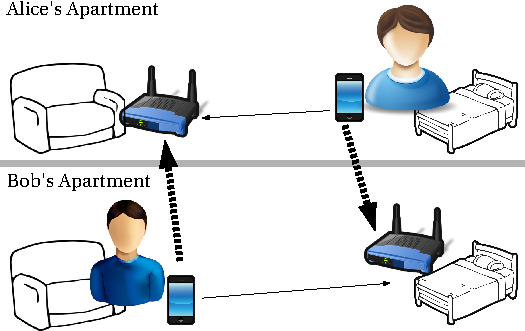
\includegraphics[width=\columnwidth]{./figures/motivation.pdf}
  \caption{\textbf{An Example of Reciprocal \wifi{} Sharing.} Solid arrows
    represent existing associations with weak signal. Dashed arrows indicate
  potentially better associations with stronger \wifi{} signal.}
  \label{fig:motivation}
\end{figure}

Nevertheless, there are several challenges in fulfilling the vision of
reciprocal \wifi{} sharing shown in Figure~\ref{fig:motivation}. First, although
the motivating example is inspired by the authors' own experience, it is not
clear how often such opportunity exists for broader range of users in real life
scenarios. Second, suppose the sharing opportunity does exist and is detected,
there is no systematic solutions to enable the \wifi{} sharing without
compromising the security and privacy of user's home network. Finally, after the
\wifi{} sharing is established, it is challenging to ensure that the
relationship remains reciprocal for both parties.

To address these challenges, we first present extensive analysis of the
\PhoneLab{} \wifi{} dataset which contains \num{21192417} scan results from 254
smartphones over 5 months (Section~\ref{sec:investigation}). The results show
that such reciprocal \wifi{} sharing opportunities does exists even in a spatial
sparse dataset. Inspired by the results, we present the design of \wisefi{}
(Section~\ref{sec:design}), a system that detects such reciprocal \wifi{}
sharing opportunities using smartphones, enables \wifi{} sharing on APs with or
without guest network support, and ensures the sharing remain reciprocal.
Finally, we discuss some open challenges in implementing such a system and point
directions for future works (Section~\ref{sec:challenges}).

\newpage
\clearpage

\section{Investigation}
\label{sec:investigation}

To investigate such reciprocal sharing opportunities, we obtain a \wifi{} scan
result dataset from \PhoneLab{} (\S\ref{subsec:phonelab}). We first develop
heuristics to identify home AP information for each device
(\S\ref{subsec:homeap}). Then we show the RSSI comparison between user's home
and neighbor APs (\S\ref{subsec:better}). Finally, we explore the reciprocal
sharing relationships in the dataset (\S\ref{subsec:reciprocal}).

\subsection{PhoneLab \wifi{} Dataset}
\label{subsec:phonelab}

\begin{table}[t]
  \begin{tabularx}{\columnwidth}{Xr}
    \toprule
    Begin & 11/7/2014 \\ 
    End & 4/3/2015 \\ 
    Duration (Days) & 147 \\ \midrule
    Participants & 254 \\
    Device Type & Nexus~5 \\ \midrule
    Scans & \num{21192417} \\
    Observed APs & \num{1197522} \\
    Used APs & \num{15668} \\ \midrule
    \wifi{} Sessions & \num{466032} \\
    Total Connection Time (Days) & \num{34721} \\
    \bottomrule
  \end{tabularx}
  \caption{\textbf{\PhoneLab{} \wifi{} Dataset Summary.} Used APs refers to the
  subset of total APs that were used by the devices participating in the study.}
  \label{tab:summary}
\end{table}

\PhoneLab{}\cite{phonelab-sensemine13} is a public smartphone platform testbed
operated at the University at Buffalo. Several hundreds of participants carry
instrumented Nexus 5 smartphones as their primary device. In particular, the
smartphone platform was modified to log each \wifi{} scan results as well as
connection events naturally generated by the Android system. Note that the same
information can also be collected by applications with appropriate permissions.
Table~\ref{tab:summary} summarizes the \PhoneLab{} \wifi{} dataset.

\wifi{} scan result represents the device's network visibility, and consists of
multiple entries---each corresponds to one \wifi{} Access Point (AP) the device
observed. The content of one entry includes: (1) beacon timestamp, (2) AP SSID
and BSSID, (3) AP channel and (4) RSSI. Additionally, the timestamp when the
scan was performed is also logged.

\subsection{Home AP Detection}
\label{subsec:homeap}

In following analysis, we focus on home \wifi{} networks which are more likely
to reveal stable and immediate reciprocal sharing opportunities. For this
purpose, we first develop several heuristics to identify the home AP for each
device in the dataset. The intuition is that the devices are most likely
connected to home AP at night. More specifically, to identify the home AP for a
device, we look at \wifi{} sessions happened during 12~AM and 4~AM and count the
number of days that the device connects to each AP during this time period. We
then identify the AP which has the largest day count as the device's home AP,
provided that the day count is larger than a threshold (30 days).

After applying the above heuristics, the home AP information of 107 devices are
identified, including 101 unique BSSIDs. There are 6 BSSIDs that are identified
as home AP for two devices. After further investigation and clarification with
\PhoneLab{} administrator, we found this is because some participants are family
members, and certain participants had device replacements during the data
collection period. In both cases, multiple devices may be associated with the
same home AP.

\subsection{\wifi{} Session Signal Strength}
\label{subsec:better}

After identified home AP information, we then ask these two questions: (1) When
the device is connected to home AP, how often does it receive a better signal
from neighbors' APs which it does not have access to? and (2) When the home AP
fails to provide best signal, is there one dominant neighbor AP among others
that provides better signal most of the time?

To answer the first question, we inspect scan results that are reported during
\wifi{} sessions with home APs. For each such scan result, we identify the
currently associated home AP, $AP_{home}$, and the AP with best RSSI among all
reported APs, denoted as $AP_{best}$. We are particularly interested in which we
refer as \textit{sub-optimal} cases, where: (1) $AP_{home} \neq AP_{best}$; (2)
the device never connects to $AP_{best}$ in the dataset; and (3) the RSSI of
$AP_{best}$ is better than $AP_{home}$ by at least certain threshold (5dBm in
our analysis). Such cases indicate that the device could potentially improve its
\wifi{} performance by connecting to neighbor APs which have better signals yet it
does not have access to. Note that here we consider RSSI as a hint in determining the
\textit{optimal} AP and it is well understood that RSSI does not directly translate
to \wifi{} performance, which we will discuss in Section~\ref{sec:challenges}.
Also note that the cases when the device are not connected to APs with best
signal due to bad roaming strategies are not interesting in the context of this
paper, and are excluded by the second condition.

\begin{figure}[t]
  \centering
  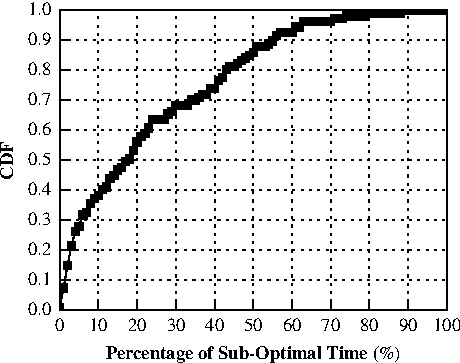
\includegraphics[width=\columnwidth]{./figures/HomeAPSessionRSSI.pdf}
  \caption{\textbf{CDF of Sub-Optimal Connection Time.}}
  \label{fig:suboptimal}
\end{figure}

We classify all scan results reported during \wifi{} sessions with home APs into
two categories: sub-optimal and the rest. For each device, we calculate the
percentage of time when the scan results indicate sub-optimal association.
Figure~\ref{fig:suboptimal} shows the CDF of such percentage for 
the 107 devices. We make several observations. First, for 80\% of the devices,
their home APs usually provides best signal (sub-optimal percentage less than
25\%). This result is not particularly surprising considering that home APs are
usually carefully positioned to try to provide good coverage. Second, we notice
that for certain number (8\%) of devices, their home APs failed to provide best
signal for more than 40\% of the time, suggesting that these users may benefit
from sharing the \wifi{} access of their neighbor APs.

Next, we are interested to see when the device is in a sub-optimal association
with its home AP, whether there exists a \textit{dominant} neighbor AP that
usually provides the best signal among other neighbor APs. If such dominant
neighbor AP exists, then by just sharing access of this one particular neighbor
AP, the device's sub-optimal association time can be largely reduced. To this
end, we look at all the scan results in sub-optimal category, and count the
number of times that each neighbor AP appears as $AP_{best}$. For each device,
we calculate the fraction of dominant neighbor AP. Figure~\ref{fig:dominantap}
shows the CDF of dominant AP fraction. For 50\% of the devices, one particular
neighbor AP contributes to more than 57\% of sub-optimal connection time,
implying that even by sharing \wifi{} access of one neighbor AP, these device's
sub-optimal connection time can be reduced by more than 57\%.

\begin{figure}[t]
  \centering
  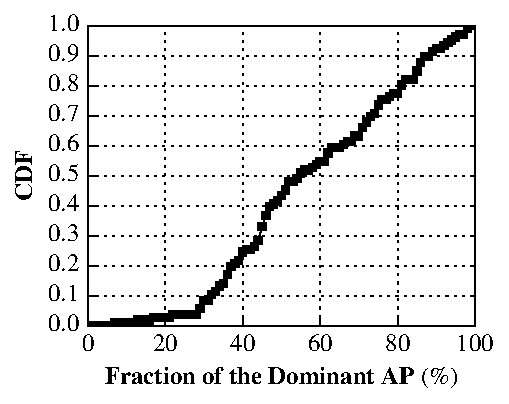
\includegraphics[width=\columnwidth]{./figures/BetterNeighborAPFigure.pdf}
  \caption{\textbf{CDF of Dominant AP Fraction.}}
  \label{fig:dominantap}
\end{figure}


\subsection{Reciprocal Sharing Opportunities}
\label{subsec:reciprocal}

Finally, we investigate the cases where two devices can obtain better signals
from each other's home AP, i.e., reciprocal sharing opportunity. We first use
scan results to establish physical neighbor information between the home APs.
Then we investigate whether reciprocal sharing opportunities exist between
neighbor APs.

To obtain the physical neighbor information, we build a home AP neighbor graph
$G_{neighbor}=(V, E)$, where $V$ is the set of all home APs, and $\langle AP_i,
AP_j \rangle \in E$ if $AP_i$ and $AP_j$ appear in the same result and both AP's
signal strengths are larger than a threshold (80~dBm), meaning $AP_i$ and $AP_j$
are physically colocated with each other. Figure 3 shows the constructed $G_{neighbor}$
from the dataset, where nodes with no edges are omitted. There are three clear
cluster of home APs. We also verified that APs in the same cluster have
different SSID and manufacturer, confirming that they are not centrally deployed
or managed.

Next, we look into potential AP sharing opportunities among colocated APs. For
each edge $\langle AP_i, AP_j \rangle \in E$, if $AP_i$'s clients receive better
(by at least 5~dBm) signals  from $AP_j$, then we draw a directed edge $\langle
AP_i\rightarrow AP_j \rangle}$, indicating that $AP_i$'s clients could
potentially benefit from sharing access of $AP_j$. We also assign a weight to
each directed edge to indicate how often such relationship happens.

The updated home AP neighbor graph is shown in Figure~\ref{fig:reciprocal}.
Sharing opportunities are sparse but exist. In particular, we observe one pair
of home APs, node 12 and 1, which exhibit \textit{reciprocal} sharing
relationships.

\sloppy{%
  We must note that \PhoneLab{} participants reside sparsely among the vast
  Buffalo area, and the above analysis is further restricted to those 
  participants that we can detect their home APs using heuristics described
  Section~\ref{subsec:homeap}. The fact that reciprocal sharing opportunities
  exist at all in such a sparse dataset is quite surprising, and motivates the
  need for a system to detect and enable such reciprocal \wifi{} sharing.
}

\begin{figure}[t]
  \centering
  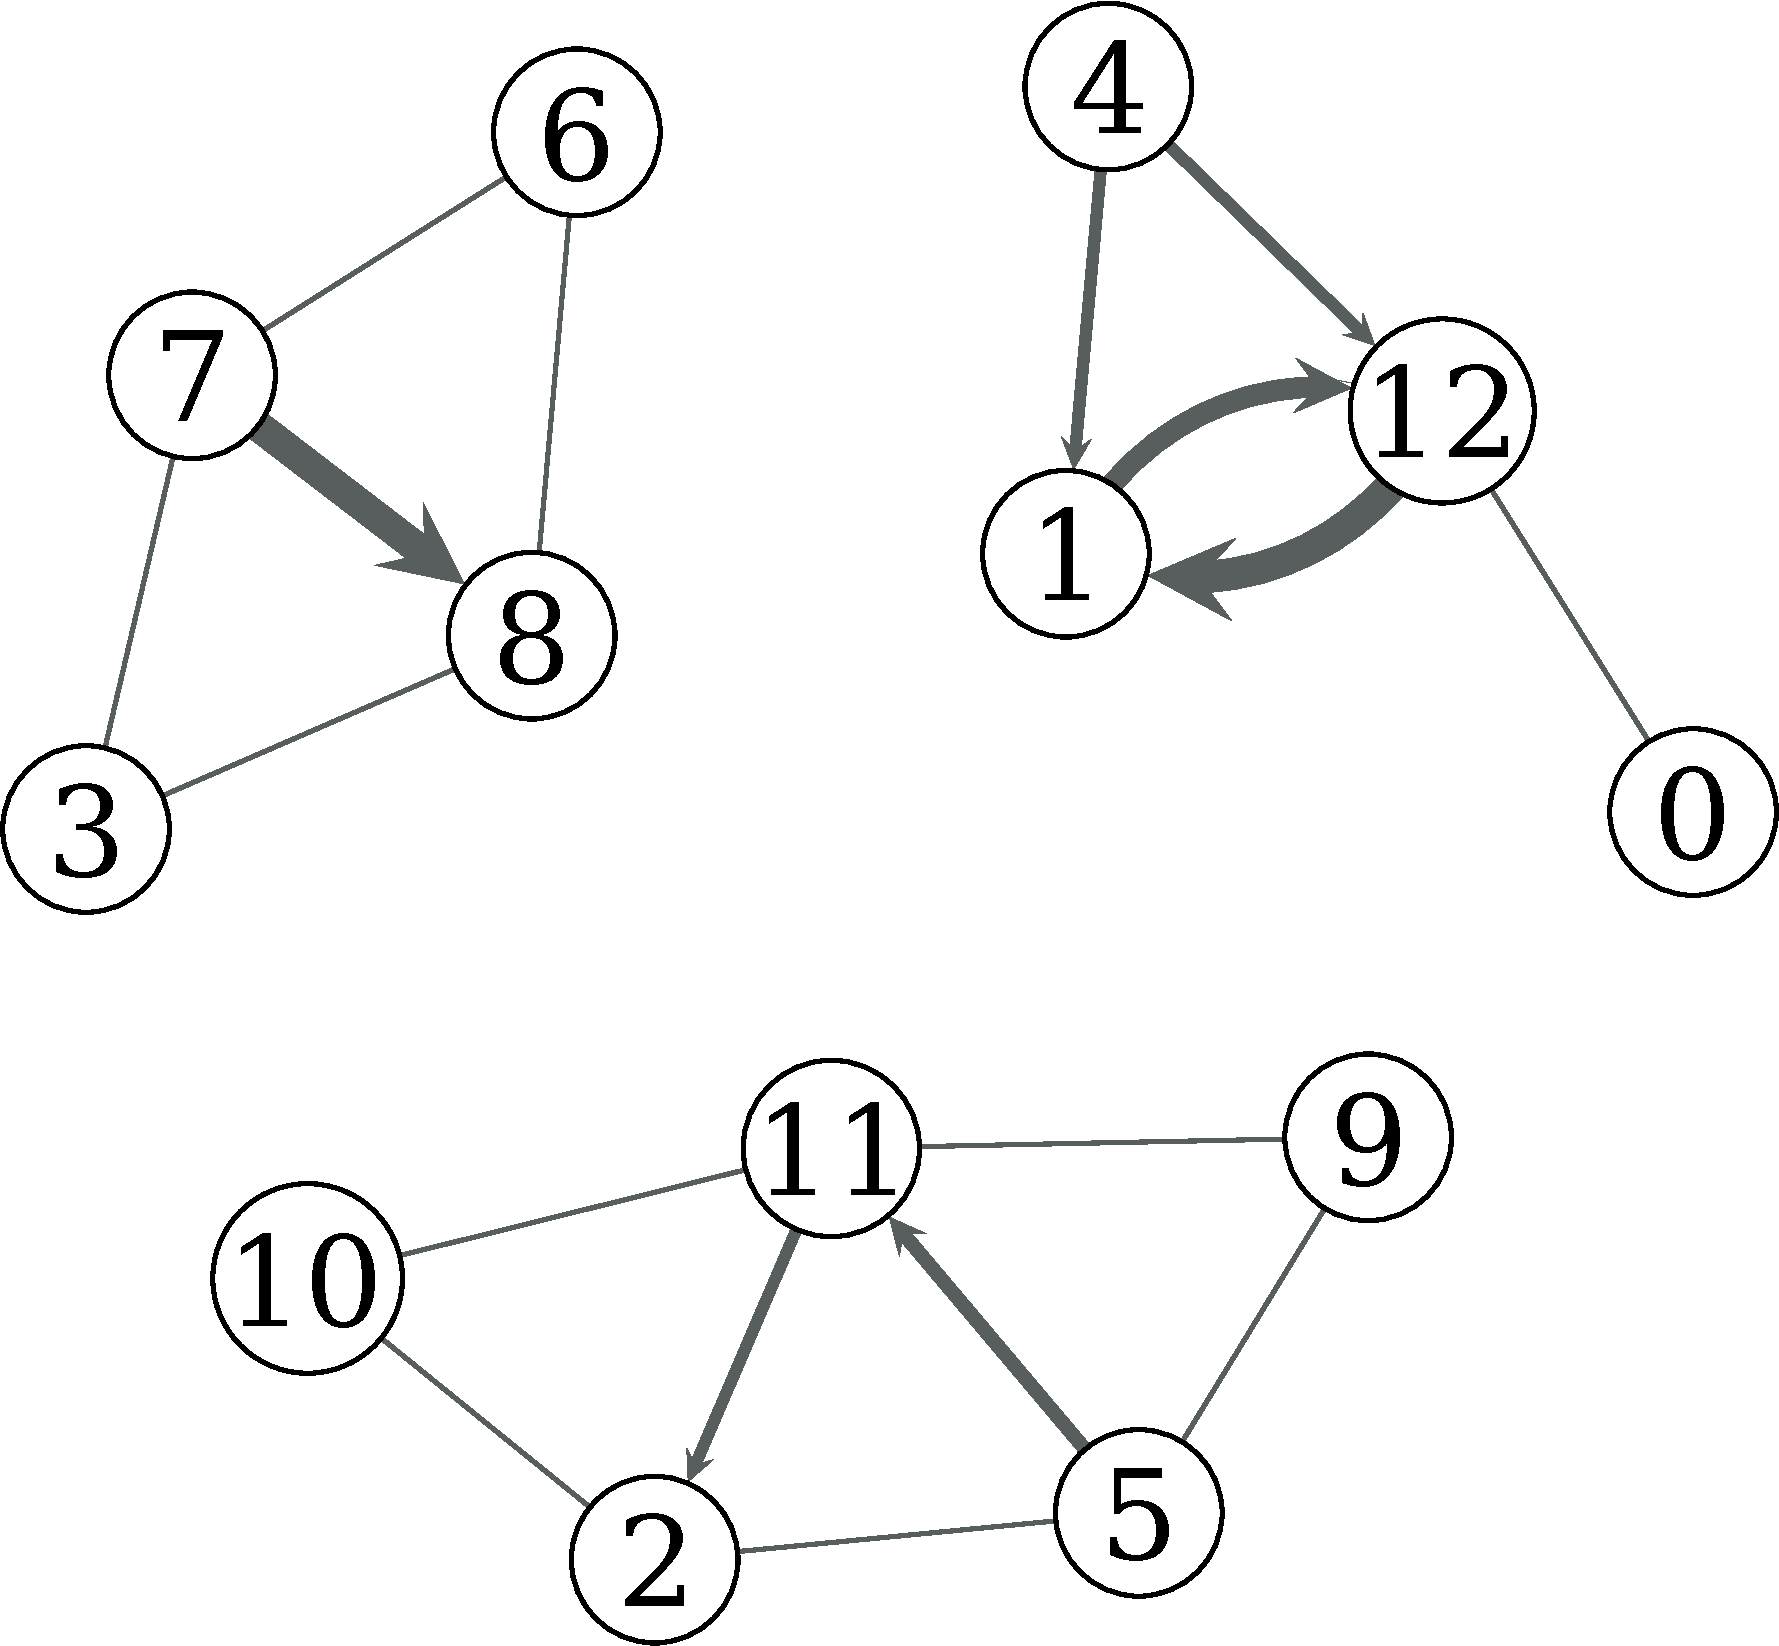
\includegraphics[width=\columnwidth]{./figures/HomeAPNeighborFigure.pdf}
  \caption{\textbf{AP Neighbor and Sharing Graph.} Edges (both directed and
    undirected) denote AP physical
    colocation relationship. Directed edges indicate AP sharing opportunities.
  Thickness of directed edges corresponds to edge weights.}
  \label{fig:reciprocal}
\end{figure}



\newpage
\clearpage


\section{System Design}
\label{sec:design}

\begin{figure*}[t]
  \centering
  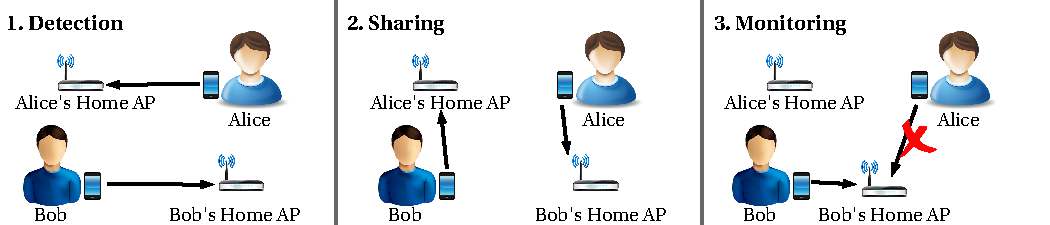
\includegraphics[width=\textwidth]{./figures/design.pdf}
  \caption{\textbf{\wisefi{} System Work Flow.}}
  \label{fig:design}
\end{figure*}

Inspired by the results of the investigation in Section~\ref{sec:investigation},
we design a system called \wisefi{} to detect reciprocal sharing
opportunities (\S\ref{subsec:detection}), enable \wifi{} sharing
(\S\ref{subsec:sharing}) and monitor the \wifi{} performance to ensure the
sharing remains reciprocal (\S\ref{subsec:monitoring}). Figure~\ref{fig:design}
shows the overall work flow of the \wisefi{} system.

\subsection{Detection}
\label{subsec:detection}

To detect reciprocal sharing opportunities, two information are required: the
home AP of the device, and neighbor APs' signal strength during \wifi{} sessions
with the home AP. A smartphone application will be deployed through app market
to collect these information. In particular, the home AP information can be
learned over a period of time using the heuristics developed in
Section~\ref{subsec:homeap}, or be resolved through user input. \wifi{} scan
results during sessions with home APs can then be logged to identify the
neighbor APs that can potentially provide better signal. Finally, these
information are uploaded and fused in \wisefi{} server to identify reciprocal
sharing opportunities as described in Section~\ref{subsec:reciprocal}.

\subsection{Sharing}
\label{subsec:sharing}

Once the reciprocal sharing opportunities are discovered, the \wisefi{} server
can then distribute such information to the smartphone clients, which will
prompt users to establish \wifi{} sharing. The sharing mechanism must meet two
goals: control and protection. First, the system should be able to control the
sharing, including granting the access of home AP to other \wisefi{} users, and
revoking the access when the reciprocal sharing opportunity no longer exists.
Second, the system should protect the home network from other \wisefi{} users by
sharing access only to the Internet, and protecting private resources such as
network printer or home network storage.

For home APs which support virtual guest network feature, the \wifi{} sharing
can be achieved by only distributing the credential of guest network to other
\wisefi{} users. Access and traffic policies can then be enforced on the guest
network to achieve control and protection. For APs without guest network
feature, however, cumbersome AP configurations may be required, such as MAC
black or white list, routing table entry. Such configurations are probably too
complicated for average users to perform. We discuss possible solutions in
Section~\ref{sec:challenges}.


\subsection{Monitoring}
\label{subsec:monitoring}

After the sharing is established, the system needs to monitor the \wifi{}
performance to ensure that the sharing remains reciprocal. There are two
reasons. First, as mentioned in Section~\ref{subsec:better}, the system uses
signal strength as a hint to identify potentially better APs. And it is well
known that signal strength does not directly translate to \wifi{} performance.
Other factors, such as AP load, modulation, interference, or \wifi{} generation,
which can not be easily detected by the smartphone, also affect the link
quality. Furthermore, last hop \wifi{} link quality does not necessarily
determines the overall end-to-end network performance. Therefore, whether
connecting to neighbor AP can indeed improve the user's network performance is
unknown until the sharing is actually established. Second, it is important to ensure that
the sharing remains reciprocal in long terms for fairness concerns. For
instance, a \wisif{} user may have a new AP deployed at home such that the home APs
always provide better or comparable \wifi{} coverage than the neighbor APs, and
there are no longer needs to share neighbor APs. The system should be able to
detect the termination of the reciprocal sharing relationship and revoke the
peer's access to the user's home AP.


\section{Open Questions}
\label{sec:challenges}

Enabling \wifi{} sharing between neighbors both touches known open issues of
cooperative \wifi{} access and brings new challenges.

As discussed in Section~\ref{subsec:sharing}, user's privacy and security can be
preserved through isolating either at network level (virtual networks) or client
level (white list vs. authenticated clients). However, it is still an open
question that whether or to what extent the user is liable to the illegal
actions, most notably copyright infringement, of the peers who share the
network.

Another challenge in establishing reciprocal \wifi{} sharing is the bootstrap
process. It is expected that during early stages of deployment, the sharing
opportunity will be sparse. Therefore, It is important to provide additional
incentives other than the benefit of \wifi{} sharing to increase the penetration
of system. One possible feature that can be added to the \wisefi{} app is to
help the user find better \wifi{} channels for their own APs. Uses who are
willing to install the app for this feature are more likely not satisfied with
their \wifi{} performance and thus have the desire of improve their network
experience by joining the reciprocal sharing relationship.

Finally, the immediate and stable sharing relationship brings new challenges to
traditional reputation or credit based peer to peer sharing mechanisms, most of
which are developed under the assumption that peers are strangers and the mutual
beneficial relationship is transient. For instance, the fairness metric of the
sharing may need to be considered over a longer time window.

\section{Related Works}
\label{sec:related}

FON~\cite{fon} is a commercial Wifi sharing network, where registered users can
roam over FON-supported Wifi networks. WLAN owners share their Wifi network
either for small money compensation, or to get Wifi access to other users when
they are way from home (roaming). FON aims at providing global Wifi sharing
community where users want to connect to others' Wifi network because they
are way from home and have no WLAN access. 

OpenWireless movement~\cite{openwireless} is a community effort for ubiquitous
Internet access. Volunteers participate the community by configuring their
\wifi{} network with open access and a special SSID, \texttt{openwireless.org}
to advertise free access. Another goal of OpenWireless is arguably preserving user's
privacy by blending the user's network activity among all other users who share
access to the open \wifi{} network.

Both FON and OpenWireless aim at sharing \wifi{} access between strangers either
through financial incentive or volunteering. Whereas in our proposal, users share
Wifi network locally (within neighbors) for better network performance, and the
sharing relationship is immediate (between two parties) and stable (physical
neighbor relationship).

\section{Conclusions}
\label{sec:conclusion}

To conclude, we explore the reciprocal sharing opportunities through extensive
analysis of the \PhoneLab{} \wifi{} dataset, and show that such opportunity does
exist despite the spatial sparsity. Inspired by the analysis results, we present
the design of \wisefi{}, a system that detects reciprocal sharing opportunities,
enable \wifi{} sharing and monitor the \wifi{} usage and performance to ensure
the sharing remains reciprocal.

We are currently implementing a \wisefi{} system prototype, which includes a
\wisefi{} Android application, dynamic AP configuration API support on OpenWRT
router platform, and \wisefi{} server powered by Django.


{\scriptsize
  \bibliographystyle{abbrv}
  \bibliography{references}
}

\end{document}
